\documentclass[11pt]{beamer}

\usetheme{metropolis}

\usepackage{graphicx}
\usepackage{physics}
\usepackage{adjustbox}
\usepackage{caption}
\usepackage{chemformula}
\usepackage{quoting}
\usepackage[style=chem-angew,backend=bibtex]{biblatex}
\bibliography{references}
%
% Choose how your presentation looks.
%
% For more themes, color themes and font themes, see:
% http://deic.uab.es/~iblanes/beamer_gallery/index_by_theme.html
%
\mode<presentation>
{
  \usetheme{default}      % or try Darmstadt, Madrid, Warsaw, ...
  \usecolortheme{default} % or try albatross, beaver, crane, ...
  \usefonttheme{default}  % or try serif, structurebold, ...
  \setbeamertemplate{navigation symbols}{}
  \setbeamertemplate{caption}[numbered]
  \setbeamerfont{footnote}{size=\tiny}
} 

\usepackage[english]{babel}
\usepackage[utf8]{inputenc}
\graphicspath{{../lectureMW/image/}}

\AtBeginSection[]{
\begin{frame}{Outline}
  \tableofcontents[currentsection]
\end{frame}
}

\title{Chapter 7: Electron Structure of the Atom}
\institute{Chemistry Department, Cypress College}
\date{November 1, 2022}

\begin{document}

\begin{frame}
  \titlepage
\end{frame}

\begin{frame}{Class Announcements}
  \textbf{Lecture}
  \begin{itemize}
  \item Share previous UCI Teaching Evaluation
  \item Hold off on reviewing the Exam and homework 8
  \item Review material from Chs 3 - 6
  \item Quiz and Homework assignment released Fri, Nov 4th at 3pm
  \end{itemize}
\end{frame}

\begin{frame}{Making the Most of It}

  Questions to consider:
  \begin{itemize}
  \item Why am I taking this course?
  \item What would I like to achieve?
  \item What methods/tools/resources work for me?
  \end{itemize}

  Your feedback, questions, participation are vital:
  \begin{itemize}
  \item Attend lectures and discussions, if possible
  \item Give on-going feedback to instructors through facial expression,
    emojis, chat, email, during office hours etc.
  \item Fill out evaluations
  \item Own your education
  \item Be proactive, do not hesitate to speak up or get help
  \end{itemize}

\end{frame}

\section{Review: Electromagnetic Radiation}

\begin{frame}{Revisit: Radiation Energy}
  \begin{center}
    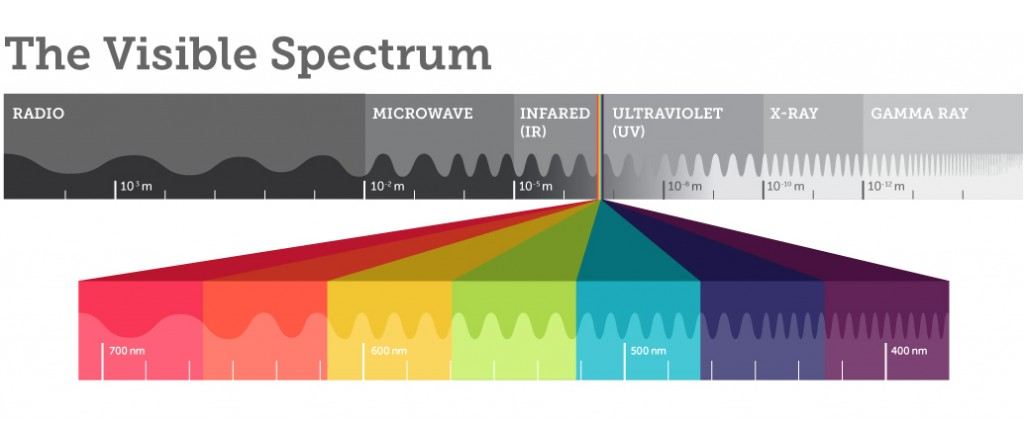
\includegraphics[width=0.85\linewidth]{visible_light}
  \end{center}
  \begin{equation}
    E = \frac{hc}{\lambda} = h\nu
    \label{eqn:photon}
  \end{equation}
  \begin{itemize}
  \item High frequency and larger wavelengths lead to higher radiation
    energy
  \item Energy are contained in packages known as photons; Eqn \ref{eqn:photon}
    computes the energy for 1 photon
  \end{itemize}
\end{frame}

\begin{frame}{Atomic Spectra}
  \centering
  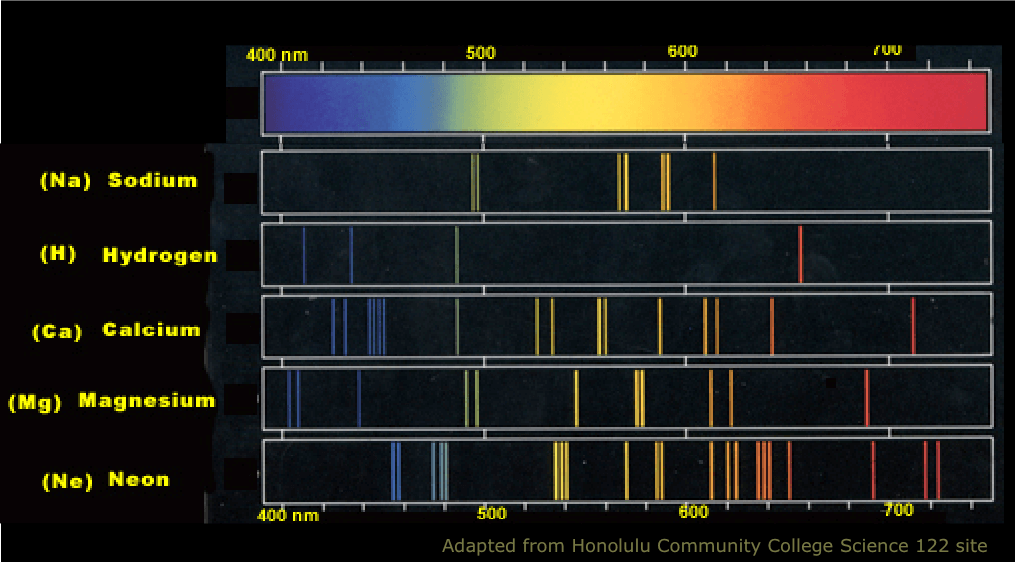
\includegraphics[width=0.85\linewidth]{cont_line}
  \begin{itemize}
  \item Continuous spectra is given at the top and
    discrete lines are emitted by atoms
  \item \textbf{Q:} Why are there discrete lines for
    the atomic spectra?
  \end{itemize}
\end{frame}

\begin{frame}{Bohr Model of the H Atom}
  \centering
  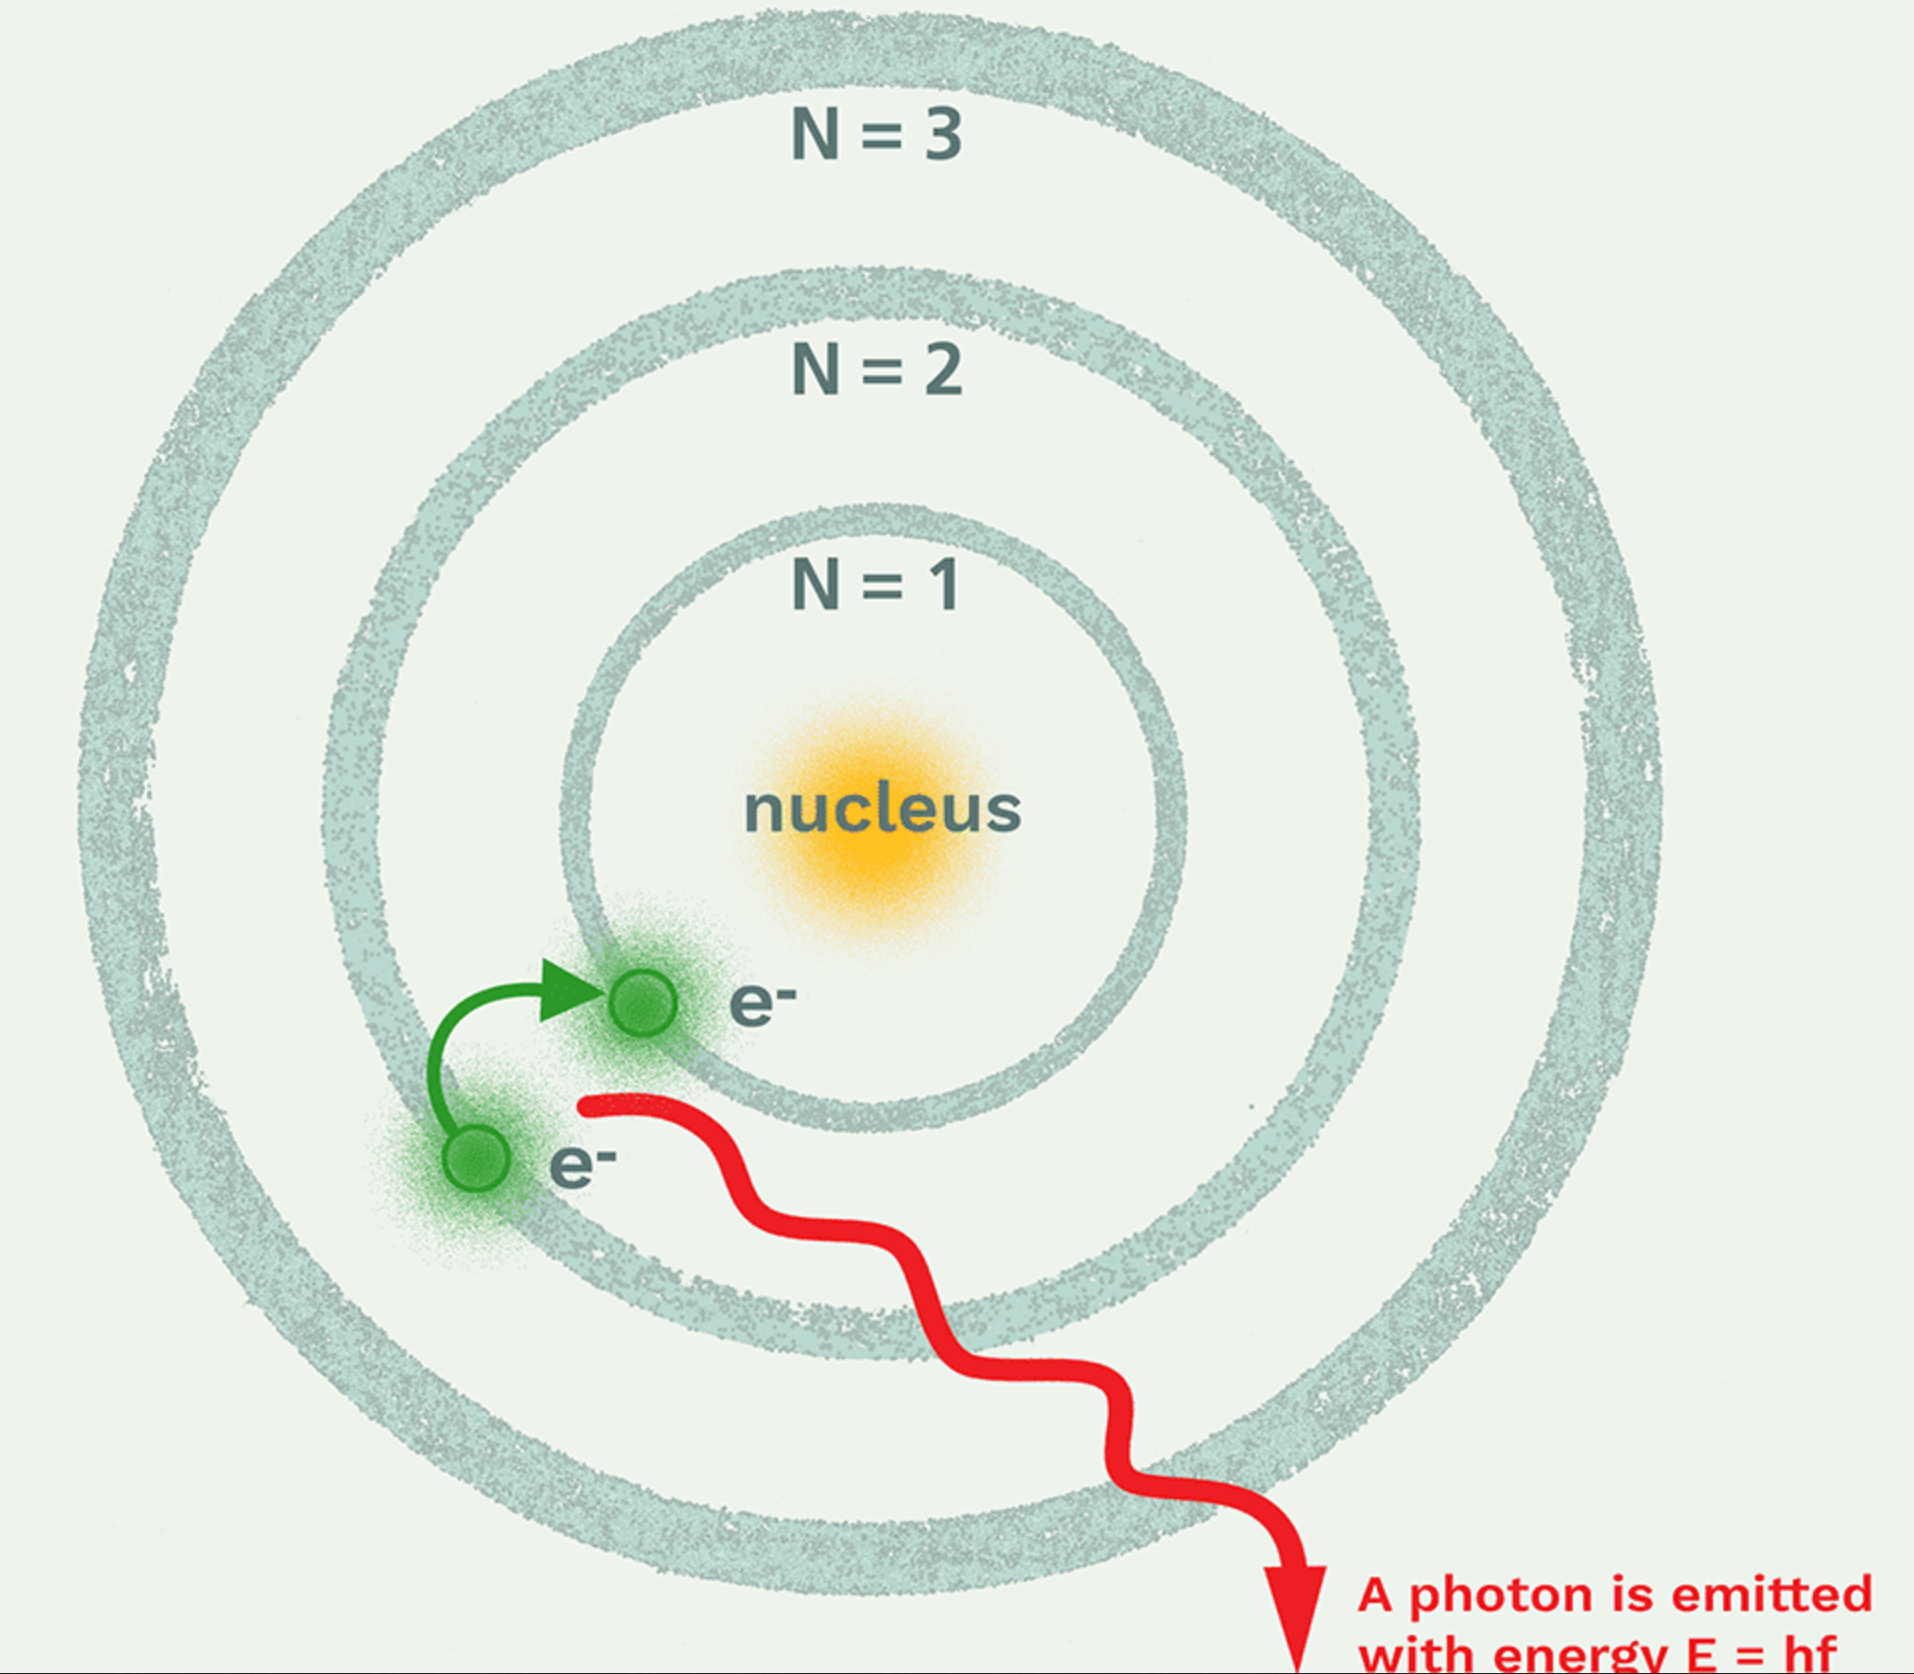
\includegraphics[width=0.55\linewidth]{bohr_model}
  \begin{align}
    \Delta E = & E_\text{final} - E_\text{initial}
  \end{align}
  Note: Keep in mind of sign conventions ($\Delta E > 0$ and
  $\Delta E < 0$)
\end{frame}

\begin{frame}{Bohr Model}
  \begin{itemize}
  \item Energy is quantized
  \item Electrons orbit the nucleus in orbits that have
    a set size and energy
  \item The energy of the orbit is related to its size; the
    lowest energy is found in the smallest orbit
  \item Radiation is absorbed or emitted when an electron
    moves from one orbit to another
  \end{itemize}
\end{frame}

\begin{frame}{Limitation of the Bohr Model}
  \begin{itemize}
  \item Violates the Heisenberg Uncertainty Principle
  \item Poor predictions regarding the spectra of larger
    atoms
  \item Does not predict the relative intensities of spectral
    lines
  \end{itemize}
\end{frame}

\begin{frame}{Example: H atom spectra}
  \textbf{Q:} According to the image, which energy level transition is
  the lowest energy? Which one has the largest energy?
  
  \begin{center}
    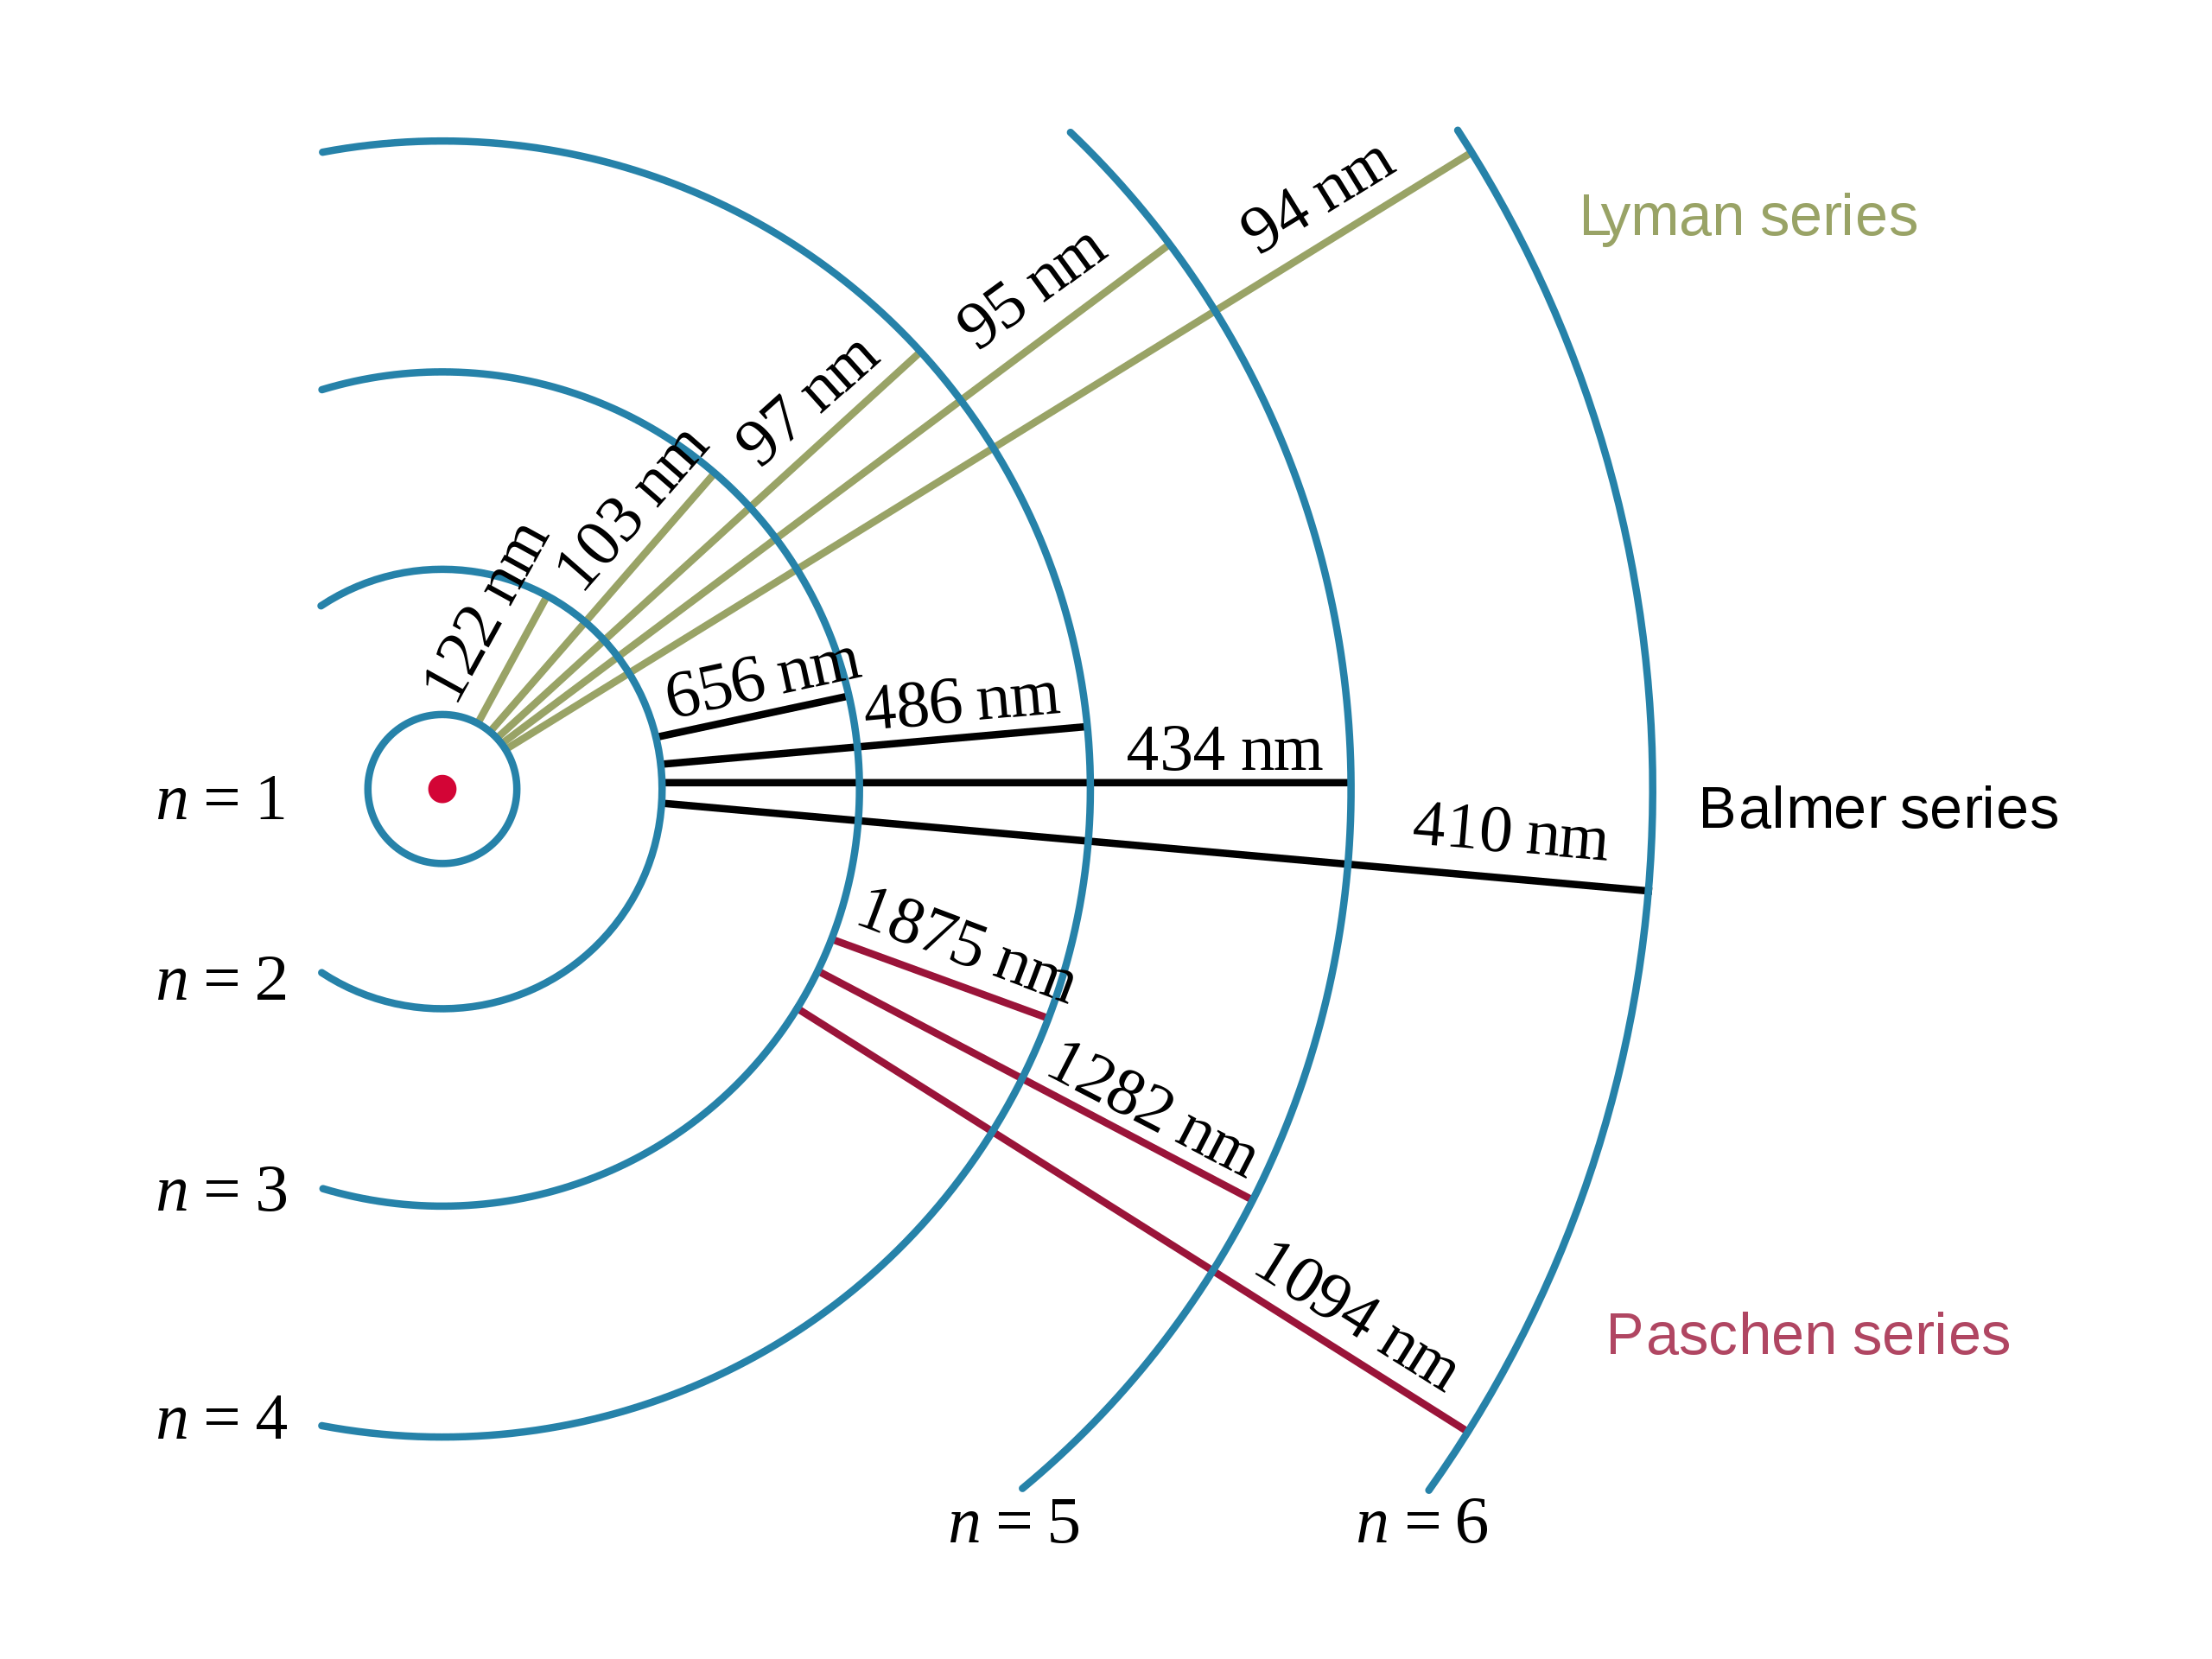
\includegraphics[scale=0.09]{h_spectra}
  \end{center}
\end{frame}

\section{Rydberg Formula}

\begin{frame}{Rydberg Formula}
  Mathematical formula to compute the wavelength between energy
  levels $n$ of a hydrogen atom

  \centering
  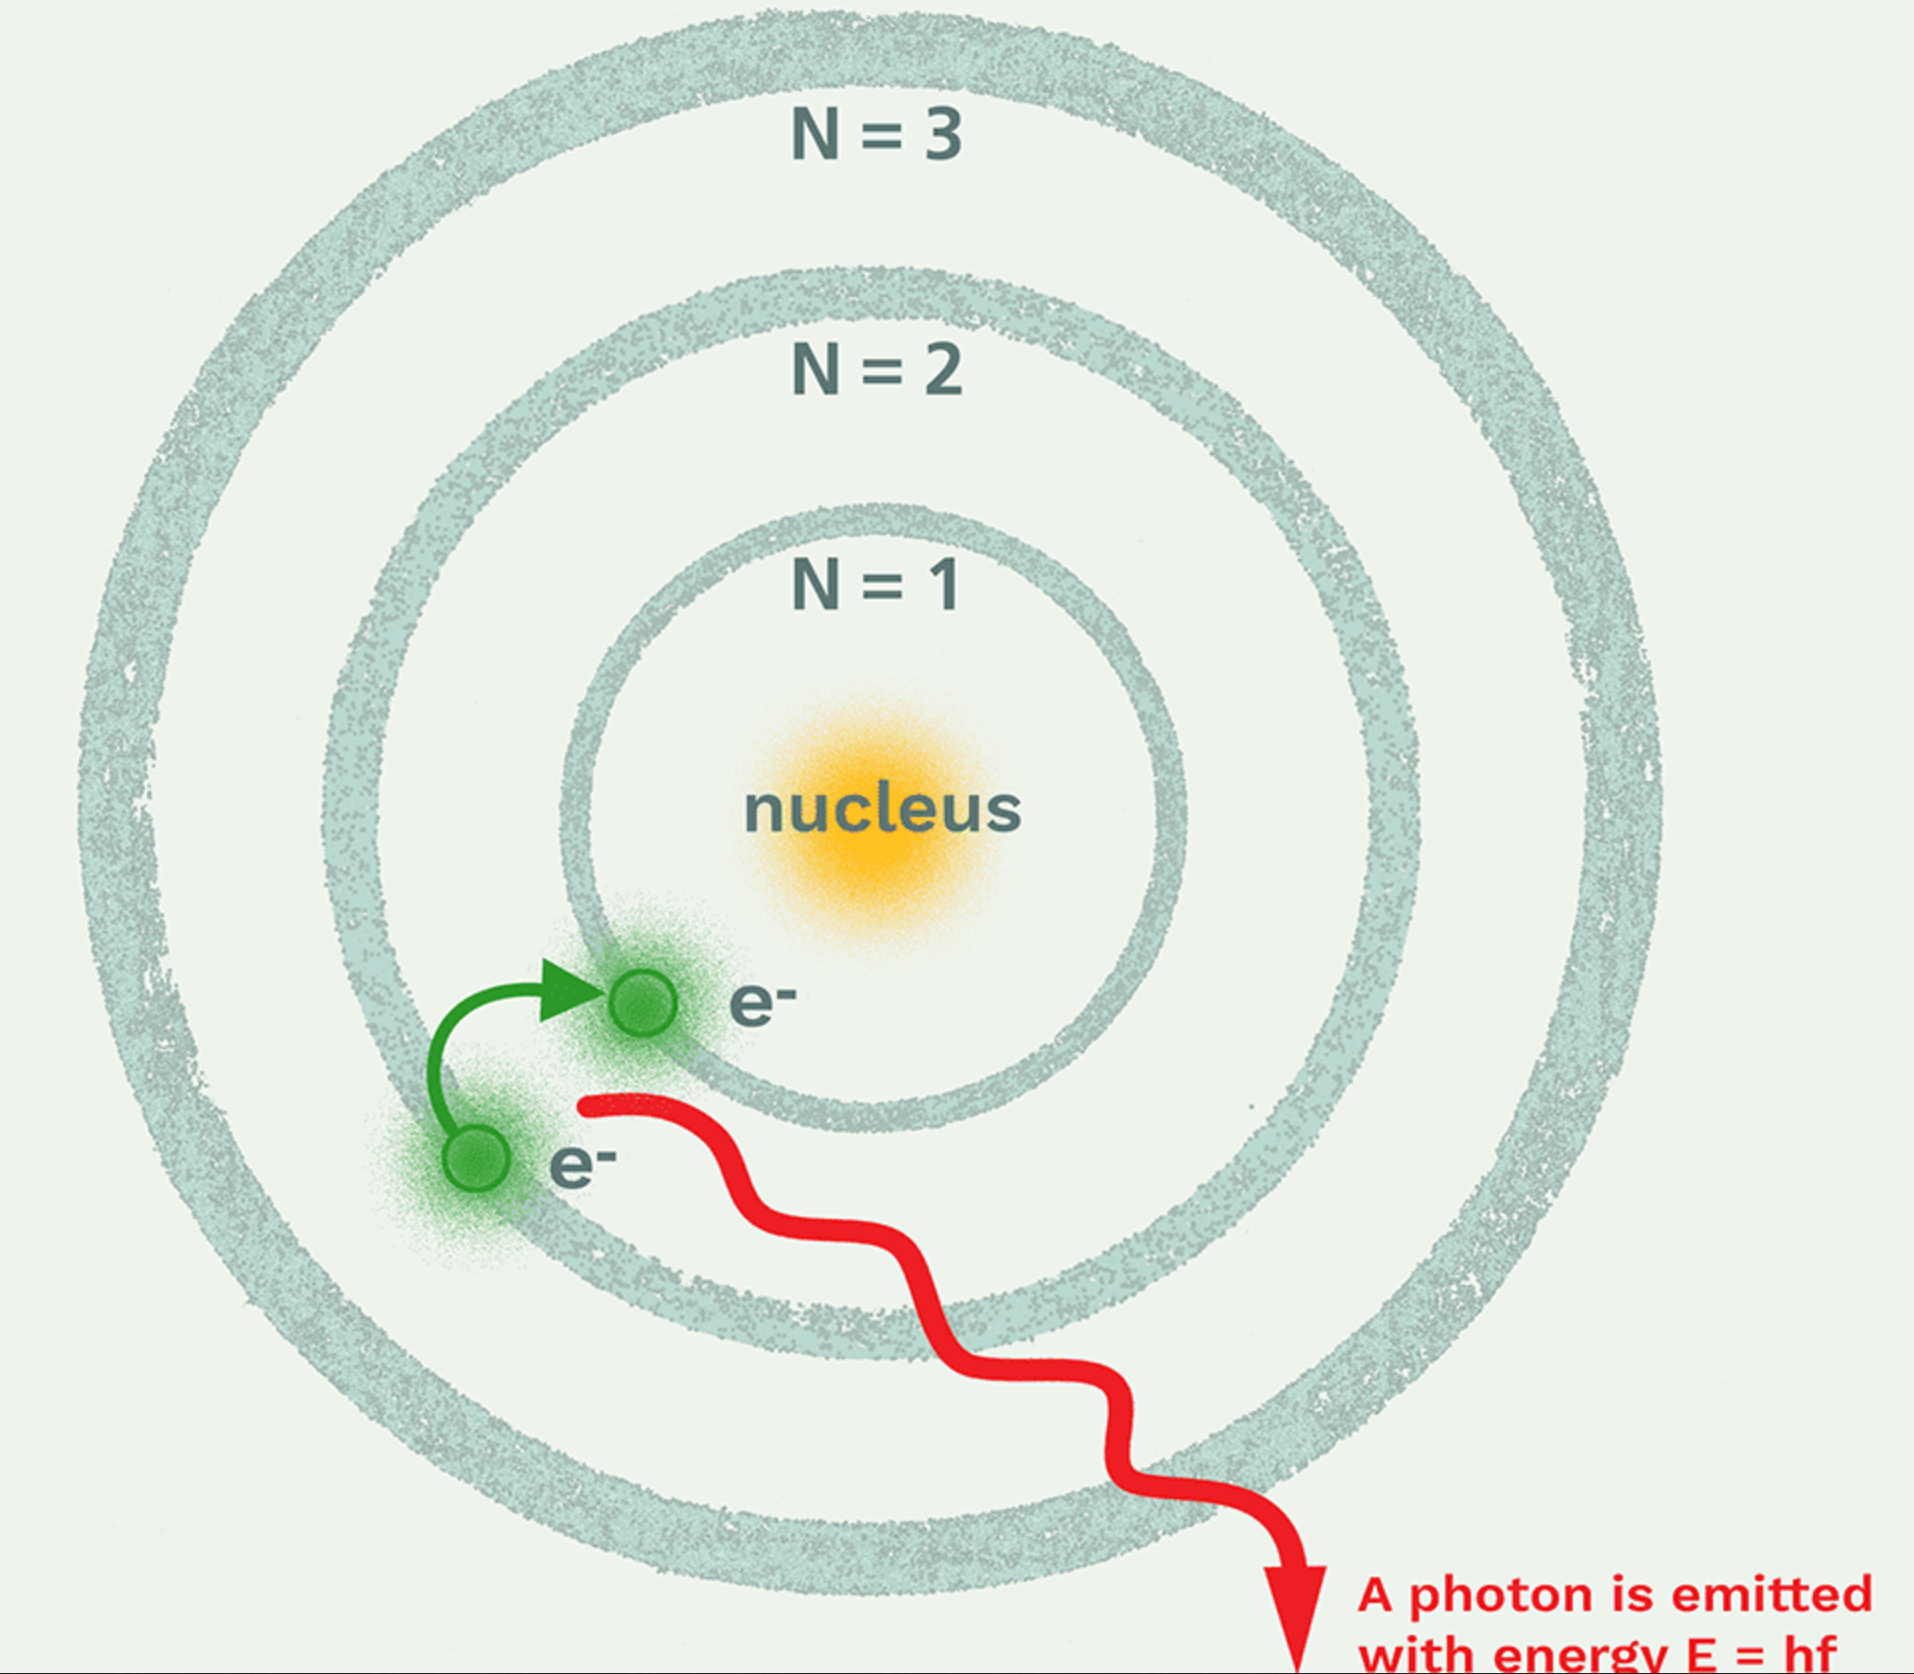
\includegraphics[width=0.55\linewidth]{bohr_model}
\end{frame}

\begin{frame}{Rydberg Formula}
  \begin{equation}
    \frac{1}{\lambda} = R\Bigg(\frac{1}{n_f^2} - \frac{1}{n_i^2}\Bigg)
  \end{equation}
  where $n_f$ and $n_i$ are the final and initial energy state,
  $\lambda$ is the wavelength, and $R$ is the Rydberg constant
  ($1.097\times 10^7$ m$^{-1}$)
\end{frame}

\begin{frame}{Practice: Using Rydberg Formula}
  Calculate the wavelength of light emitted when a hydrogen atom relaxes
  from $n = 6$ to $n = 2$. Is this light in the visible region of
  electromagnetic spectrum? If so, what color is it?
  \onslide<2->{
  \begin{center}
    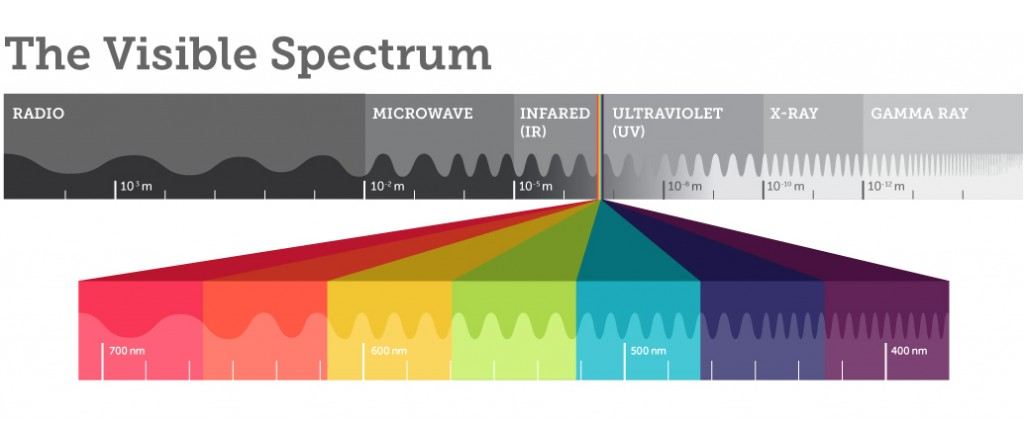
\includegraphics[width=1\linewidth]{visible_light}
  \end{center}
  }
  \vfill
\end{frame}

\begin{frame}{Practice: Using Rydberg Formula}
  What is the energy of the wavelength when a hydrogen atom relaxes
  from $n = 6$ to $n = 2$?
  \vspace{1in}
  \vfill
\end{frame}

\section{Review: Identifying Types of Compounds and Naming Compounds}

\begin{frame}{Properties of Ionic Compounds}
  \begin{center}
    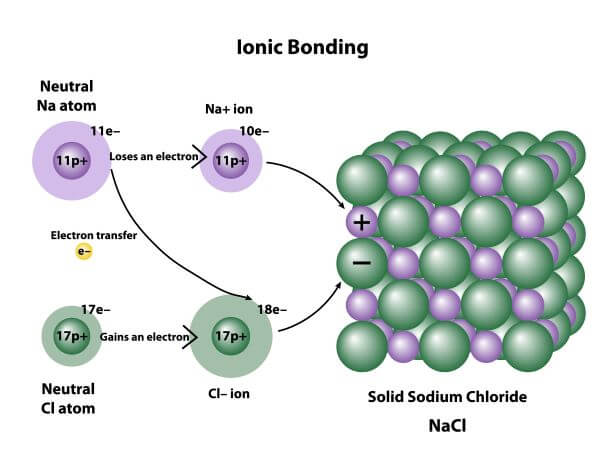
\includegraphics[width=0.6\linewidth]{Ionic-bond-example}
  \end{center}
  \vspace{-0.3in}
  \textbf{Ionic Compounds}
  \begin{itemize}
  \item Highly conductive and strong electrolyte - ability to
    carry electricity (electrons)
  \item High melting and boiling points, high density
  \end{itemize}
\end{frame}

\begin{frame}{Properties of Molecular Compounds}
  \begin{center}
    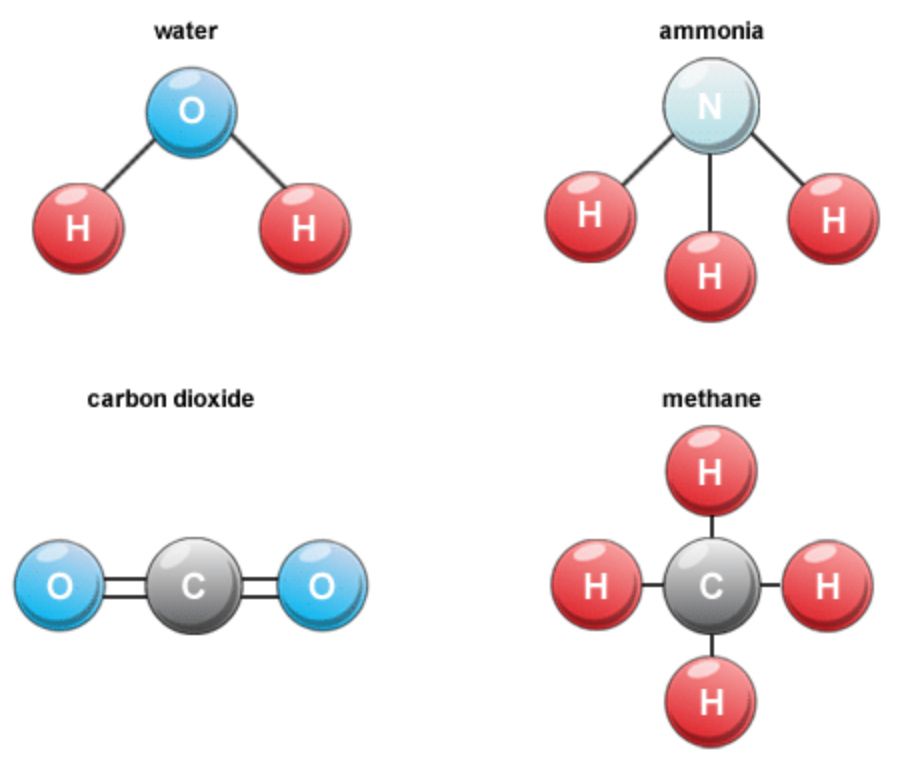
\includegraphics[width=0.6\linewidth]{molec_example}
  \end{center}
  \vspace{-0.3in}
  \textbf{Molecular Compounds}
  \begin{itemize}
  \item Not conductive and weak electrolyte
  \item Low melting and boiling points, low density
  \end{itemize}
\end{frame}

\begin{frame}{Practice: Determine the following as Ionic or Molecular}
  \begin{itemize}
  \item CaCl$_2$
  \item Ca$_3$P$_2$
  \item MgO
  \item FeCl$_2$
  \item Co$_2$O$_3$
  \item V$_2$O$_5$
  \item NH$_4$F
  \item H$_3$PO$_4$
  \end{itemize}
\end{frame}

\subsection{Ionic Compounds}

\begin{frame}{Naming Ionic Compounds}
  The metal cation is named first, followed by the nonmetal anion.
  The word ion is dropped from both parts.

  \centering
  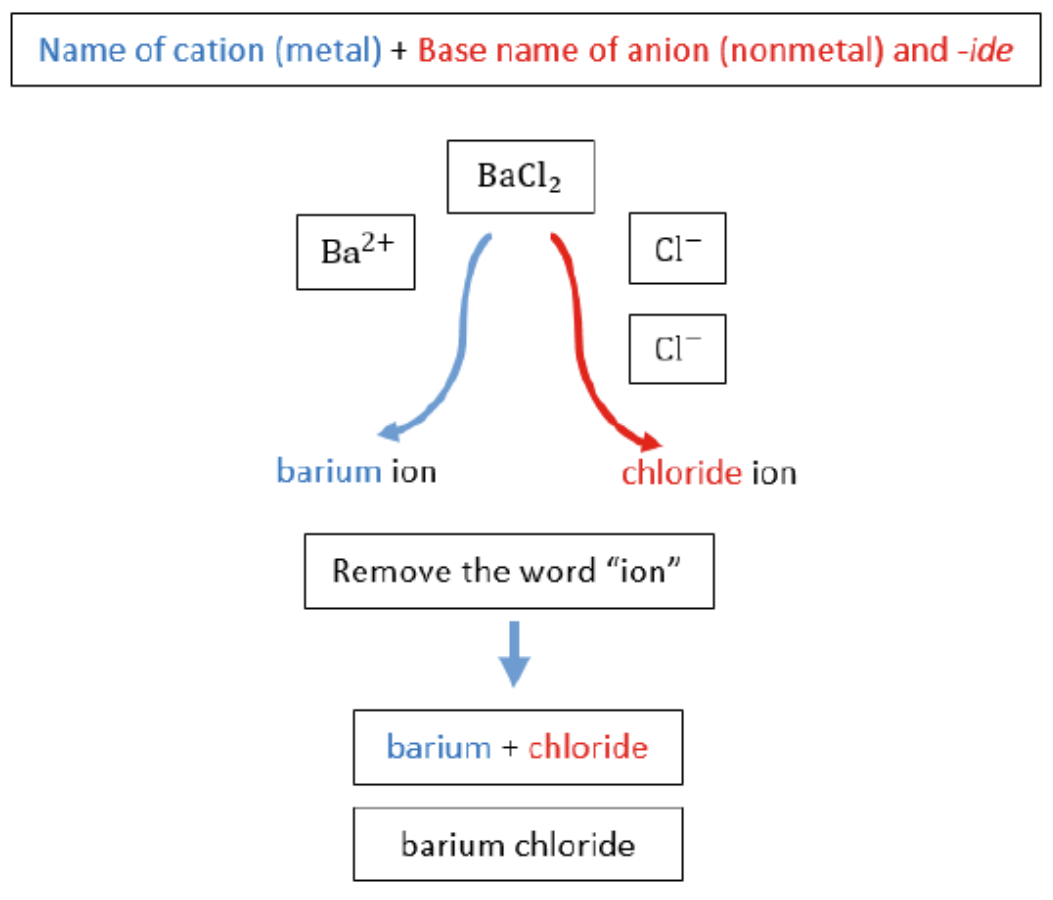
\includegraphics[width=0.7\linewidth]{barium_examp.png}
\end{frame}

\begin{frame}{Special: Certain metals}
  \centering
  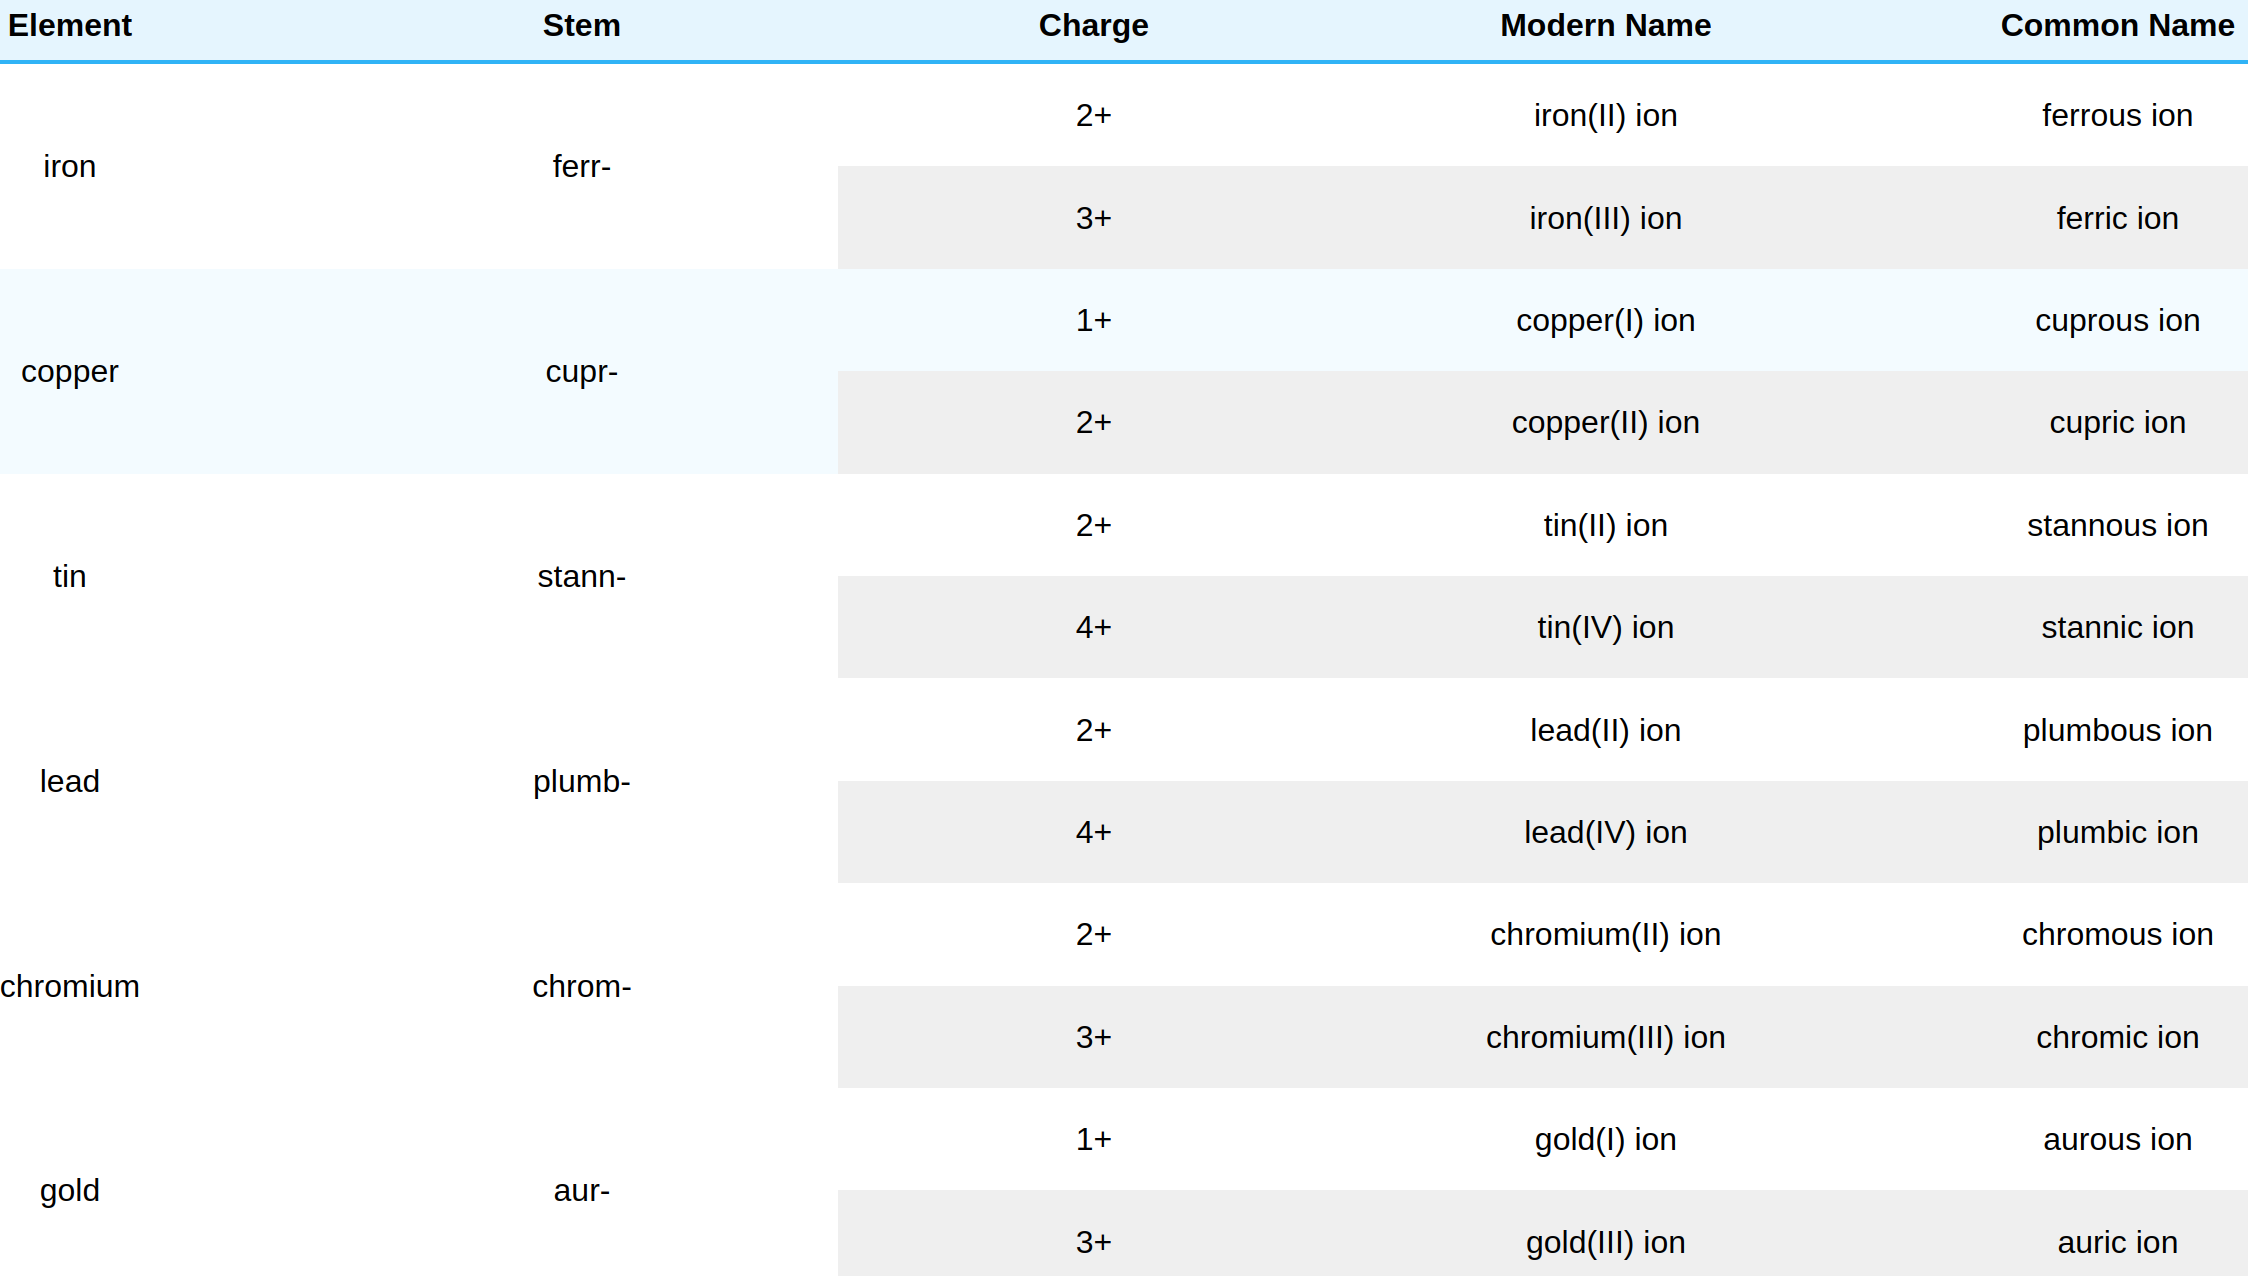
\includegraphics[width=\linewidth]{ions_names}
\end{frame}

\begin{frame}{Practice: Name the Ionic Compound}
  \begin{itemize}
  \item CaCl$_2$
  \item Ca$_3$P$_2$
  \item MgO
  \item FeCl$_2$
  \item Co$_2$O$_3$
  \item V$_2$O$_5$
  \end{itemize}
\end{frame}

\begin{frame}{Practice: Determining Molecular Formula}
  \begin{itemize}
  \item Vandium(V) Oxide
  \item Chromium(VI) Oxide
  \item Iron(III) Oxide
  \item Sodium chloride
  \item Barium fluoride
  \item Lead(IV) fluoride
  \item Ammonium sulfate
  \item Calcium phosphate
  \item Aluminum perchlorate
  \item Sodium bicarbonate
  \end{itemize}
\end{frame}

\subsection{Molecular Compounds}

\begin{frame}{Naming Molecular Compounds}
  \begin{center}
    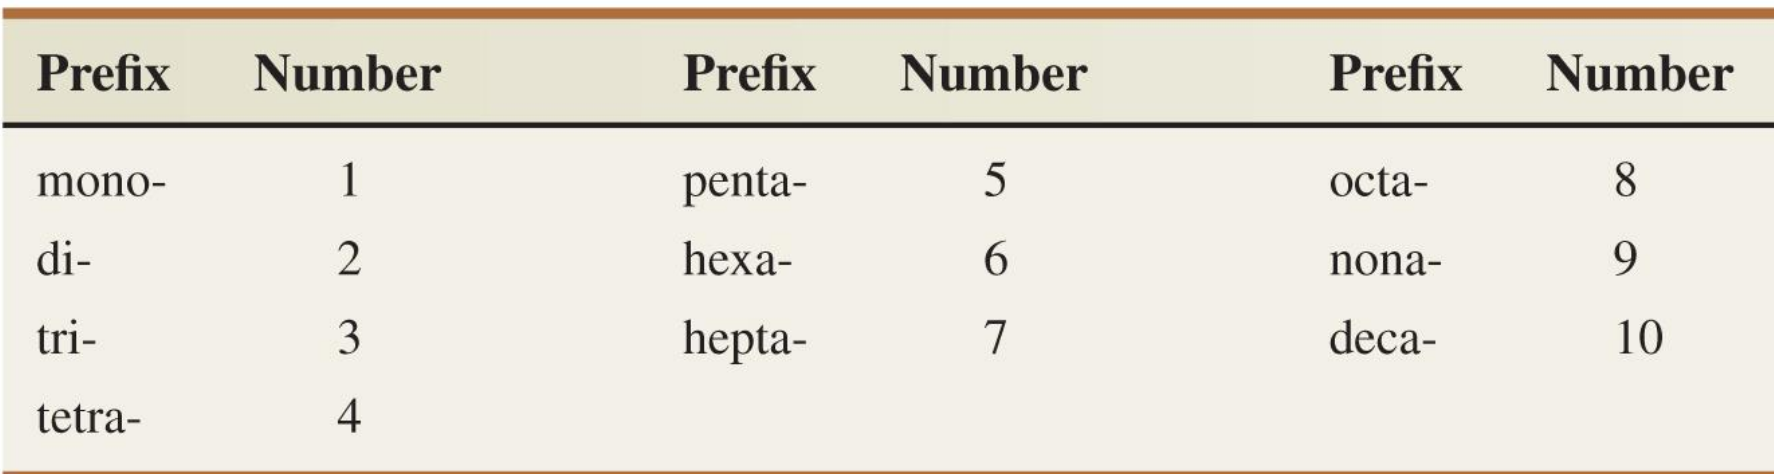
\includegraphics[width=\linewidth]{prefix_name}
  \end{center}
  
  \begin{enumerate}
  \item Use numerical prefix for the element (usually ignore the first
    when using ``mono'')
  \item Add ``-ide'' to the second element
  \end{enumerate}
\end{frame}

\begin{frame}{Practice: Naming Binary Molecular Compounds}
  \begin{itemize}
  \item H$_2$O
  \item N$_2$O$_4$
  \item CO
  \item CH$_4$
  \item PF$_5$
  \item BF$_3$
  \item SiO$_2$
  \item XeF$_4$
  \end{itemize}
\end{frame}

\begin{frame}{Practice: Determining Molecular Formula}
  \begin{itemize}
  \item Sulfur trioxide
  \item Nitrogen trihydride
  \item Dihydrogen monoxide
  \item Carbon tetrafluoride
  \item Selenium dichloride
  \item Dinitrogen pentaoxide
  \item Sulfur hexafluoride
  \item Phosphorus trifluoride
  \end{itemize}
\end{frame}

\subsection{Acids and Bases}

\begin{frame}{Naming Acids and Bases}
  \begin{center}
    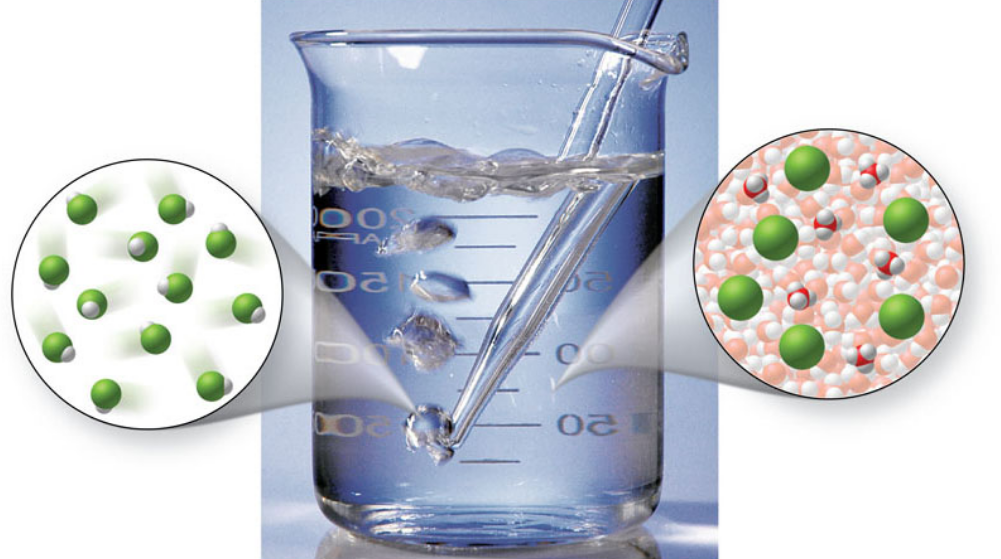
\includegraphics[width=0.5\linewidth]{acid_base}
  \end{center}

  \begin{enumerate}
  \item If anion ends in ``-ide,'' add ``hydro'' before the
    root of the anion name followed by ``-ic acid''
  \item If anion ends in ``-ate,'' use the root of the anion
    name followed by ``-ic acid''
  \item If anion ends in ``-ite,'' use the root of the anion
    name followed by ``-ous acid''
  \end{enumerate}
\end{frame}

\begin{frame}{Practice: Naming the Acid}
  \begin{itemize}
  \item HCl
  \item HNO$_3$
  \item H$_2$CO$_3$
  \item H$_2$SO$_3$
  \item H$_3$PO$_4$
  \item HClO$_2$
  \item HBr
  \item HNO$_2$
  \item H$_2$SO$_3$
  \item H$_2$S
  \end{itemize}
\end{frame}

\begin{frame}{Practice: Determining Molecular Formula}
  \begin{itemize}
  \item Cloric acid
  \item Phosphoric acid
  \item Sulfurous acid
  \item Hydrosulfuric acid
  \item Chromic acid
  \item Nitric acid
  \item Hypochlorous acid
  \item Hydrobromic acid
  \end{itemize}
\end{frame}

\end{document}
